\chapter{Conclusion and Future Work}
\label{chp:6:ConcFutu}

In this final chapter, the study will be finalized by summarizing it under the conclusion section, and its possible extensions will be discussed in the future work section.

\section{Conclusion}
\label{sec:6.1:Conc}

Increased Internet usage made email a popular medium for communication because of its low cost, quick turnover and the flexibility of connectivity through the use of mobile devices. The benefits of email communication also attracted researchers to use it as a data collection medium to explore, describe, and explain things by communicating with a large group of people.
\vspace{1cm}

However, the nature of communication with large groups is different compared to small ones due to the required effort in personalizing messages according to its respective recipient. As a result, researchers tend to write more generic emails, ignoring recipient-specific details. Researchers investigated many response rate influences, and addressed that personalization of the message content is an important factor in increasing the response rate \citep{Dillman1991,Schaefer1998}. Messages that are not personalized results in a low response rate for the answers expected from the recipients. As a result, this may end up with a nonresponse error.
\vspace{1cm}

Nonresponse error has been considered as a major problem by many researchers, because of the tendency of some of the respondents as a part of a large group who fails to respond might result in a biased estimate for the proper representation of the population. Hence, it affects the outcome of a research \citep{Bogen1996}.
\vspace{1cm}

For this reason, the researchers investigated possible theories regarding the reason behind proper personalization's effect on the response rate. While \cite{DillmanDonA.SmythJoleneD.Christian2009} emphasized the social exchange theory since the personalization of emails helps build a connection between the respondents and the researcher, \cite{Barron2002} stressed on the diffusion of responsibility theory, which talks about the awareness of the availability of the other volunteers will result in a higher utility of not volunteering.
\vspace{1cm}

The researchers conducted studies on investigating the diffusion of responsibility. \cite{Barron2002} showed that the number of replies where they used a single email address in the "To" field got a 20\% higher response rate and the number of "very helpful" replies was 187\% higher compared to the replies they got when they used groups of email addresses. In the study of \cite{Selm2006}, the recipients showed privacy concerns when the header of the email contained all the email addresses of the other respondents explicitly.
\vspace{1cm}

Other researchers investigated the social exchange theory. \cite{Heerwegh2005} applied personalized salutations in the the emails, and got a 6.9\% higher login rate for the provided survey link in the email compared to the non-personalized group in their study. In the study of \cite{Joinson2007}, when the level of authority or status of the sender was used with the personalized salutation, they got a 53.4\% response rate while non-personalized salutations with a neutral power of the sender status got a 40.1\% response rate.
\vspace{1cm}

Even though personalization of emails helps increase the response rates, \cite{DillmanDonA.SmythJoleneD.Christian2009} emphasized that an overwhelmed personalization can also result to a low response rate. Hence, only the adequate amount of personalization and its appropriateness should be considered for personalizing emails. In addition to this, experienced email users can easily notice if a message is manually written by a person, or if it is computer generated. Therefore, it is hard for the digital world to achieve authentic personalization, and achieving such level of personalization requires getting to know each recipient very well.
\vspace{1cm}

To understand what existing applications offer in support for personalized mass email communication, \ac{CRM}, Help Desk, and Email Marketing applications were evaluated in chapter \ref{chp:3:EvalExisAppl}. Several features of these applications are considered to be helpful to researchers for their mass email communication. Some of these features are the following:

\begin{compactitem}
	\item Storing client related information extracted from conversations in \ac{KVP}s.
	\item Integration with popular email clients such as Gmail.
	\item Importing recipient lists from third-party applications.
	\item Assigning emails to a recipient profile.
	\item Using dynamic variables in the emails to be replaced by their values.
	\item Assigning a help desk ticket to an assistant.
	\item Reusability of an existing email as a template.
\end{compactitem}
\vspace{1cm}

Moreover, none of the available products indicated above offers these mentioned features in helping a personalized mass email communication all under a single product and some of these features needs additional effort to use since their application focus is not a mass email communication. Therefore, this study came up with an initial solution as a prototype featured in chapter \ref{chp:4:InitIdeaProt}. The prototype supported following features to help a researcher reach large groups of people in a personalized way with less effort:

\begin{compactitem}
	\item Kept extracted information in \ac{KVP}s along with the recipient messages.
	\item Used dynamic variables to personalize the salutations of emails.
	\item Allowed to reuse earlier sent messages as a template.
	\item Provided a tree structure to get an overview of the state and flow of the conversation with the used templates.
\end{compactitem}
\vspace{1cm}

Even though the prototype provided the above mentioned features in support to a personalized mass email communication, we moved the prototype from its origin product, EmailValet, to a new project after the informal user test with an organization who performs mass email communication regularly at Stanford University. The user test ended up with new features, and it helped us realize the drawbacks of the existing EmailValet as an email client we used for the prototype.
\vspace{1cm}

The improved requirements after user test brought up the final solution in chapter \ref{chp:5:FinaSolu}, and its features in support for mass email communication as follows:

\begin{compactitem}
	\item Recipients' information can be synchronized to the Myriad system through a Google Spreadsheet to remove the effort on importing and exporting recipients' information from the researchers.
	\item A researcher can assign assistants to an email campaign for them to interact with the flow of a mass email communication with tasks such as extracting information from incoming answers, proofreading the primary researcher's replies before sending them or even composing replies to those answers.
	\item Extracted respondents' information can be recorded to the recipients' respective profiles in the \ac{KVP}s during the whole state of a campaign. 
	\item Those recorded \ac{KVP}s can be used as dynamic variables in personalizing the content of the emails.
	\item Reusability of exiting emails and getting an overview of the state of the conversation.
	\item Provided a decision-making mechanism to automate earlier decisions on sending out emails in a user verified manner.
	\item Provided visual cues to notify users on the current state of communication with individual recipients, and suggesting potential action based on the previous decisions of the user.
	\item All conversations and extracted information of each recipient are provided under a single view respectively to conveniently reach all the necessary information to write recipient specific personalized emails.
 \end{compactitem}

Considering the features gathered in the final solution, we provided a workflow to the researchers aimed to help reduce the amount of time needed in personalizing the content of the emails. Considering the Effort vs. Personalization chart from figure \ref{fig:ChartEffortCustom} after the final solution, it could be replaced in a way as shown in figure \ref{fig:drawingEfforPersonalizationAnnotations}, compared with other products in the market focusing on email communication and data collection. Considering the user feedbacks and the amount of people actively using Myriad during its beta stage, we believe that Myriad was able to bridge the gap in achieving the gold standard of effort vs. personalization, as annotated in the figure.
\vspace{1cm}

Finally, possible future work on enhancing the existing solution and remove the known existing restrictions are to be discussed in the next section.

\begin{figure}[htbp]
	\centering
	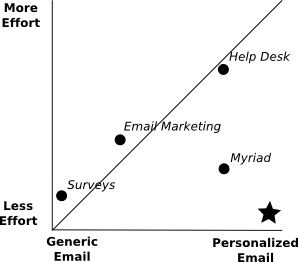
\includegraphics[width=.55\textwidth]{imgs/drawingEfforPersonalizationAnnotations.png}
	\caption[Effort vs Personalization and the Comparison of Available Solutions]{Effort vs Personalization and the Comparison of Available Solutions}
	\label{fig:drawingEfforPersonalizationAnnotations}
\end{figure}

\section{Future Work}
\label{sec:6.2:FutuWork}

The provided assistant support in the final solution helps researchers share certain tasks in extracting information from emails, proofreading the primary researcher's replies before sending them, compose replies to recipients' emails, and to verify the rule-based actions before they are acted upon.
\vspace{1cm}

Along with the assistant support, the system could also provide an option to allow a crowd of anonymous workers to perform the tasks of assigned assistants, as a crowd assistant. If the system would be able to provide the required functions to allow the involvement of crowd assistants, the decisions on the possible tasks in a mass email communication can be done by anonymous crowd workers.
\vspace{1cm}

\cite{Surowiecki2005} stated that under the right conditions, groups can be remarkably smart, and even smarter than the smartest person within them. Therefore, if you try to solve a complicated problem or try to make a decision, the best thing to do is to ask a group instead of trying to find an expert. Therefore, taking advantage of crowd assistants can minimize the work a researcher needs to do in a personalized mass email communication.
\vspace{1cm}

Another improvement could be about the dynamic variables in the messages. \ac{KVP}s were used in the messages as dynamic variables to personalize the content of the messages as described in section \ref{subsec:5.2.4:CompEmaiMess}. However, when communicating with larger groups of people, some \ac{KVP}s might not be applicable to some recipients, or other irregular \ac{KVP}s needs to be used to personalize messages for some recipients in a large group. When we reviewed available products in the market as featured in chapter \ref{chp:3:EvalExisAppl}, Zendesk solved this issue by adding conditional logic to the dynamic variables, as illustrated in listing \ref{lst:MailChimCondMergTags}. Such extension would be an option for Myriad to avoid creating additional email templates for closely similar emails, with minor changes on \ac{KVP}s.
\vspace{1cm}

In chapter \ref{chp:3:EvalExisAppl}, we saw that that \ac{CRM} applications provide task management options to remind users about upcoming tasks. For example, Highrise allows association of a task to an email to let users easily browse through the source of the task in the provided task list. Currently, Myriad users can maximize the use of the \ac{KVP}s for the same purpose by adding a key named "task" and a value according to the recipients. However, this contradicts with one design principle, separation of concerns, since the logic behind the \ac{KVP}s is to store extracted information from the recipients' emails and use them to personalize emails. Besides, \ac{KVP}s connected to the recipients' profile in a campaign is not useful in adding task messages related to a message of a recipient. Therefore, the task management feature in Myriad could be useful for researchers in attaching reminder messages as a task along with the recipients' messages, and a list of these tasks are shown at the main page of a campaign.
\vspace{1cm}

One Myriad user mentioned about the email editor and its attachment handling in the user testimonials, as shown in listing \ref{lst:Testimonial1}. Currently, Myriad provides an \ac{HTML} editor to compose an email; however, it does not provide an option for adding attachments. This is due to the limited time for development, and adding this feature was not considered as a priority at the time of the development since users can still use Gmail in composing an email, and Myriad will able to import it, together with its attachment. Therefore, a better \ac{HTML} editor with an email attachment feature would necessary to accomplish all email composing tasks inside the Myriad system.
\vspace{1cm}

Next improvement could be on the visualization tree of the communication state and flow. The current visualization tree's nodes are arranged according to email templates and their order in the communication. However, a user can opt to create all email templates at the beginning of a campaign and use them according to the recipients answer later on. In this case, all the created templates at the beginning of the campaign will be considered as individual root nodes of a tree, losing the hierarchical structure in visualizing the communication state. Therefore, the possible improvement should let Myriad allow the rearrangement of those nodes in the visualization tree, together with a drag-and-drop ability for each node.
\vspace{1cm}

Lastly, a better workflow can be implemented in the future by the provided rules created according to the decision on sending emails. Currently, Myriad saves filtering conditions of a recipient search as a rule in sending emails the next time, without having the need to search for matching conditions of the recipients again. This feature is quite unintuitive, since when user decides to browse through the rules view, no defined rules will be shown, unless the user uses the provided filtering options in getting a subset of the recipient list and then send an email to the recipients afterwards. To make this feature more intuitive and better define the workflow of a mass communication before-hand, Myriad could offer an option on creating rules right under the rules view. With this, a researcher can easily create the rules and assistants can verify and send emails according to the matching rules, or even opt to automate the process by the provided option under the rules view.

 